\section{Statistical Perspective}

In this part we will explore a statistical perspective on supervised learning by estimating the data distribution and then deriving a decision rule from the distribution. This allows us to express prior knowledge about the data. We start with the fundamental assumption that our data is generated iid. by some unknown distribution, note that this assumption is often violated in practice:
$$(x_i, y_i) \sim p(x, y)$$

We want to find a hypothesis $f: X \mapsto Y$ that minimizes the \textbf{expected loss / prediction error / population risk} (over all possible data):
$$R(f) = \int p(x,y) \ell(y, f(x)) dxdy = \E_{x,y}[\ell(y, f(x))]$$

We have already seen that the \textbf{empirical risk / training error} $\hat{R}_D(f)$ often underestimates the population risk. But by the law of large numbers we have that empirical risk approaches the population risk. We call this difference $|\hat{R}_D(f) - R(f)|$ the \textbf{generalization error} w.r.t. $f$.

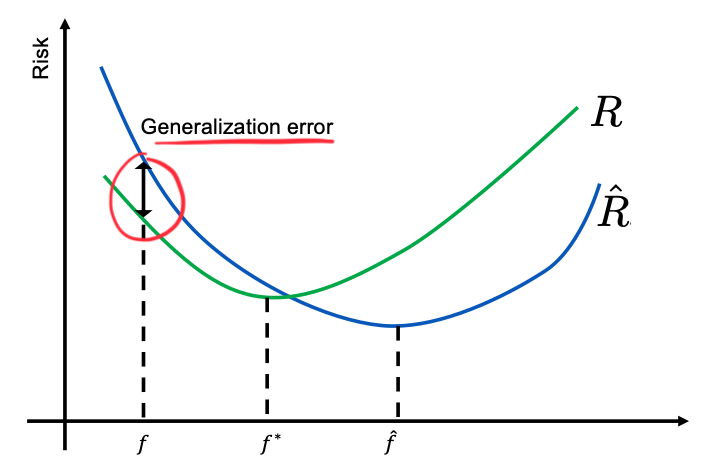
\includegraphics[width=\columnwidth]{risk.png}

\subsection{Optimal Predictor for the Squared Loss}

The population risk for the squared loss is:
$$R(f) = \E_{x,y}[(y - f(x))^2]$$

Suppose we knew $p(x,y)$ which $f$ minimizes the population risk?
\begin{align*}
	f^* &= \min_f \E_{x,y}[(y - f(x))^2] \\
	&= \min_f \E_x[\E_y[(y - f(x))^2 \; | \; X=x]] \\
	&= \E_x[ \min_f \E_y[(y - f(x))^2 \; | \; X=x]]
\end{align*}

Now we focus on the inner part, suppose we are given a fixed $x$:
$$f^*(x) = \argmin{\hat{y}} \; \E_y[(\hat{y} - y)^2 \; | \; X = x)] = \E[y \; | \; X = x]$$

We therefore have shown that $f^*$ minimizing the population risk is given by the conditional mean, which can be calculated by:
$$f^*(x) = \E[y \; | \; X = x] = \int y \cdot p(y \; | \; x) dy$$

Note that we only need the conditional distribution $p(y \; | \; x)$ and not the full joint distribution $p(x, y)$. Thus one strategy is for estimating a predictor from training data is to estimate the conditional distribution $\hat{p}(y \; | \; x)$ and then use it to predict labels via the conditional mean. \medskip

One common approach to estimate the conditional distribution is to choose a particular parametric form and then estimate the parameters $\theta$ with the maximum (log) likelihood estimation:
\begin{align*}
	\theta^* &= \argmax{\theta} \; \hat{p}(y_1, ..., y_n \; | \; x_1, ..., x_n, \theta) \\
	&= \argmin{\theta} \; - \sum_{i=1}^n \log p(y_i \; | \; x, \theta) 
\end{align*}

\subsubsection{Example: Conditional Linear Gaussian}

Let us look at the case where we make the assumption that the noise is Gaussian. We have $y = f(x) + \epsilon$ with $\epsilon \sim \mathcal{N}(0, \sigma^2)$ and $f(x) = w^\top x$. Therefore the conditional probability is:
\begin{center}
	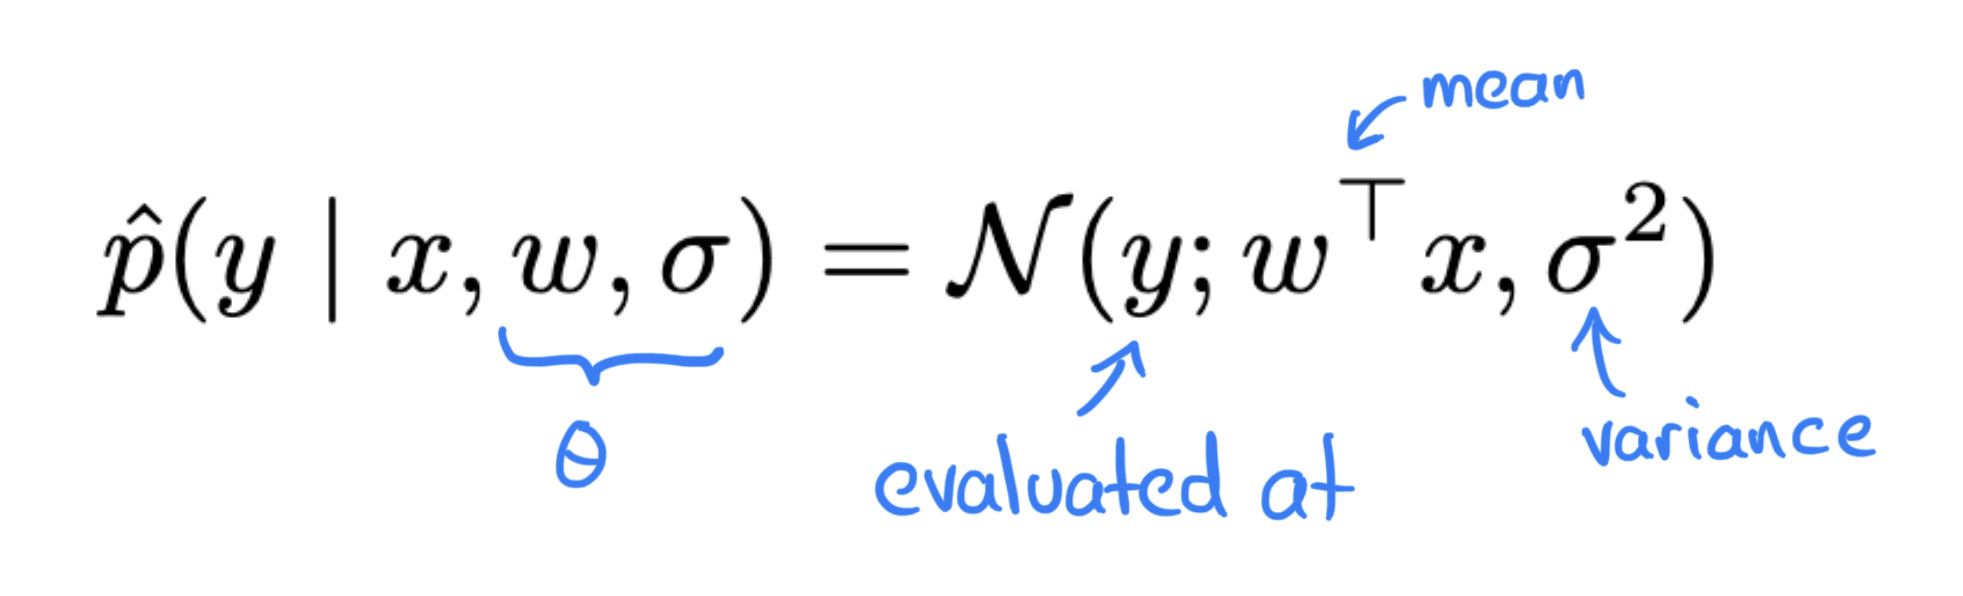
\includegraphics[width=0.7\columnwidth]{gaussian-conditional-prob.jpeg}
\end{center}

Then we can find the optimal $\hat w$ by using the definition of the normal distribution (some steps are left out):
\begin{align*}
	\hat w &= \argmax{w} \; \hat p(y_{1:n} \; | \; x_{1:n}, w, \sigma) \\
	&= \argmin{w} \sum_{i=1}^n - \log \mathcal{N}(y_i \; | \; x_i, w^\top x, \sigma^2) \\
	&= \argmin{w} \sum_{i=1}^n (y_i - w^\top x_i)^2
\end{align*}

Therefore we have shown that under the conditional linear Gaussian assumption, the MLE is equivalent to the least squares estimation.

\subsubsection{Bias-Variance Tradeoff}

Recall that the following hold:
$$\text{Prediction Error} = \text{Bias}^2 + \text{Variance} + \text{Noise}$$

Where we have:
\begin{itemize}
	\item \textbf{Bias}: Excess risk of best model considered compared to minimal achievable risk knowing $p(x,y)$
	\item \textbf{Variance}: Risk incurred due to estimating model from limited data
	\item \textbf{Noise}: Risk incurred by optimal model (irreducible error)
\end{itemize}

The MLE for linear regression is unbiased, further it is the minimum variance estimator among all unbiased estimators. However, we have also seen that it can overfit.

\subsection{Maximum a Posteriori Estimate}

It is often favourable to introduce some bias (make assumptions) to reduce variance drastically. One such assumption could be that the weights are small. We can capture this assumption with a Gaussian prior $w_i \sim \mathcal{N}(0, \beta^2)$. Then, the posterior distribution of $w$ is given by:
\begin{align*}
	p(w \; | \; \bar x, \bar y) &= \frac{p(w, \bar x, \bar y)}{p(\bar x, \bar y)} \\
	&= \frac{p(w, \bar y \; | \; \bar x) \cdot p(\bar x)}{p(\bar y \; | \; \bar x) \cdot p(\bar x)} \\
	&= \frac{p(w) \cdot p(\bar y \; | \; w, \bar x)}{p(\bar y \; | \; \bar x)}
\end{align*}

Hereby we used that $w$ is apriori independent of $\bar x$ (note that $\bar x = x_{1:n}, \bar y = y_{1:n}$). Now we want to find the maximum a posteriori estimate (MAP) for $w$:
\begin{align*}
	\hat w &= \argmax{w} \; p(w \; | \; \bar x, \bar y) \\
	&= \argmin{w} \; - \log p(w) - \log p(\bar y \; | \; w, \bar x) + \log p(\bar y \; | \; \bar x) \\
	&= \argmin{w} \; \frac{\sigma^2}{\beta^2} ||w||_2^2 + \sum_{i=1}^n(y_i - w^\top x_i)^2
\end{align*}

Which is exactly the same as ridge regression with $\lambda = \frac{\sigma^2}{\beta^2}$. More generally, regularized estimation can often be understood as MAP inference, with different priors (= regularizers) and likelihoods (= loss functions).

\subsection{Statistical Models for Classification}

We now want to do the same risk minimization for classification. The population risk for the 0-1 loss is:
$$R(f) = \mathbb P[y \neq f(x)] = \E_{x,y}[\mathbb I_{y \neq f(x)}]$$

Suppose we knew $p(x,y)$ which $f$ minimizes the population risk?
\begin{align*}
	f^*(x) &= \argmin{\hat y} \; \E_y [\mathbb I_{y \neq \hat y} \; | \; X = x] \\
	&= \argmax{\hat y} \; p(\hat y \; | \; x)
\end{align*}

This hypothesis $f^*$ minimizing the population risk is given by the most probable class, this hypothesis is called the Bayes' optimal predictor for the 0-1 loss.

Similar to the regression we can now look at logistic regression and assume that we have iid. Bernoulli noise. Therefore the conditional probability is:
$$p(y \; | \; x,w) \sim \text{Ber}(y; \sigma(w^\top x))$$

Where $\sigma(z) = \frac{1}{1 + \exp(-z)}$ is the sigmoid function. Using MLE we get:
\begin{align*}
	\hat w &= \argmax{w} \; p(\bar y \; | \; w, \bar x) \\
	&= \argmin{w} \sum_{i = 1}^n \log (1 + \exp(-y_i w^\top x_i))
\end{align*}

Which is exactly the logistic loss. Instead of solving MLE we can estimate MAP, e.g. with a Gaussian prior:
\begin{align*}
	\hat w &= \argmax{w} \; p(w \; | \; \bar x, \bar y) \\
	&= \argmin{w} \; \lambda ||w||_2^2 + \sum_{i = 1}^n \log (1 + \exp(-y_i w^\top x_i))
\end{align*}






